\documentclass[10pt,a4paper]{article}

\usepackage[utf8]{inputenc}
\usepackage[T1]{fontenc}
\usepackage{amsmath,amssymb,amsfonts}
\usepackage{graphicx}
\usepackage{hyperref}
\usepackage{algorithm}
\usepackage{algpseudocode}
\usepackage{multicol}
\usepackage{geometry}
\usepackage{cite}
\usepackage{authblk}
\usepackage{amsmath, mathtools, empheq}

% Page layout
\geometry{margin=2cm}

% Title page
\title{\Large\textbf{TPTT: Transforming Pretrained Transformers into Titans}}
\author{\large Fabien Furfaro\thanks{\texttt{fabien.furfaro@gmail.com}}}
\date{\large 2025}

\begin{document}

\maketitle

\begin{abstract}
    \textbf{Background:} Large language models (LLMs) based on the Transformer architecture have achieved remarkable success in natural language processing, but their computational and memory demands remain a significant challenge, especially for long-context inference. 
    
    \textbf{Methods:} We propose TPTT (Transforming Pretrained Transformers into Titans), a novel framework that augments pretrained Transformer models with efficient linearized attention mechanisms and advanced memory management. TPTT introduces techniques such as Memory as Gate (MaG) and mixed linearized attention (LiZA), and is fully compatible with the Hugging Face Transformers library, enabling parameter-efficient fine-tuning (LoRA) without full retraining.
    
    \textbf{Results:} Experiments on the MMLU benchmark with $\sim$1B parameter models demonstrate substantial improvements in both efficiency and accuracy. For instance, Titans-Llama-3.2-1B achieves a 20\% increase in Exact Match (EM) over its baseline.
    
    \textbf{Conclusions:} TPTT enables scalable, robust adaptation of existing LLMs to long-context tasks, outperforming recent state-of-the-art methods in both performance and resource utilization. Source code and package are available at \url{https://github.com/fabienfrfr/tptt} and \url{https://pypi.org/project/tptt/}.
\end{abstract}
    


\begin{figure}[ht]
    \centering
    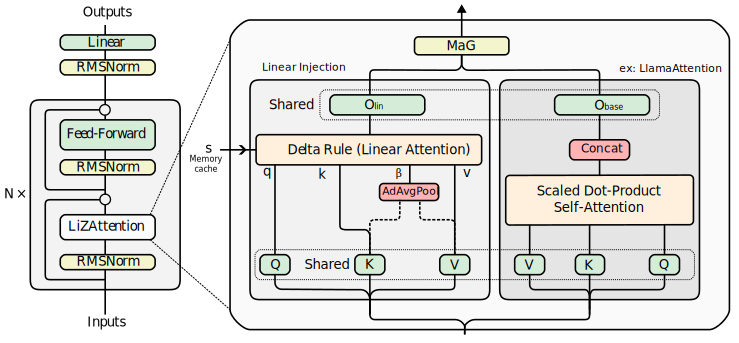
\includegraphics[width=0.8\linewidth]{fig.pdf}
    \caption{Overview of the TPTT architecture. On the left, the diagram illustrates a decoder-only architecture where linear attention is injected in parallel of vanilla attention (LiZAttention). On the right, the detailed architecture of the linearized attention mechanism is depicted, highlighting the shared weights for query (Q), key (K), value (V), and output (O) projections. It also shows the management of the state memory (S) and the combination of outputs through the Memory as Gate (MaG) weighting mechanism. The state can be unlinear between chunk. The diagram emphasizes the integration of linearized attention mechanisms and advanced memory management techniques, such as DeltaProduct and AdaptativeAvgPool1D, contributing to processing and output generation.}
    \label{fig:approach_overview}
\end{figure}


\section{Introduction}

Transformer-based large language models (LLMs) have revolutionized natural language processing (NLP), achieving state-of-the-art results across a wide range of tasks, from text generation to code synthesis~\cite{vaswani2017attention, mann2020language}. However, the quadratic complexity of the self-attention mechanism in both computation and memory remains a major limitation, particularly for applications requiring long-context inference, such as document understanding, multi-turn dialogue, and scientific reasoning.

Recent research has sought to address these challenges through a variety of approaches. Efficient attention mechanisms~\cite{katharopoulos2020transformers, yang2024parallelizing} aim to reduce the computational burden by approximating or restructuring the attention operation, while recurrent and memory-augmented architectures~\cite{mercat2024linearizing, behrouz2024titans} introduce internal memory to better capture long-range dependencies. At the same time, parameter-efficient fine-tuning techniques such as LoRA~\cite{hu2022lora} have made it feasible to adapt large pretrained models to new domains or tasks without the need for full retraining.

Despite these advances, most existing solutions require substantial architectural changes or retraining from scratch, limiting their applicability to already deployed or proprietary models. There remains a need for methods that can efficiently endow existing LLMs with long-context and memory-augmented capabilities, while preserving their pretrained knowledge and minimizing adaptation cost.

\textbf{In this paper, we introduce TPTT (Transforming Pretrained Transformers into Titans), a practical and scalable framework for upgrading pretrained Transformers with efficient linearized attention and advanced memory mechanisms.} Our approach integrates techniques such as Memory as Gate (MaG) and mixed linearized attention (LiZA), inspired by recent advances in memory-augmented neural architectures~\cite{behrouz2024titans}. TPTT is fully compatible with the Hugging Face Transformers library and leverages parameter-efficient fine-tuning (LoRA), enabling seamless adaptation of any causal LLM to long-context tasks.


\textbf{Our main contributions are:}


\begin{itemize}
    \item We propose TPTT, a framework for augmenting pretrained Transformers with linearized attention and memory gating, requiring minimal changes to the original architecture.
    \item We introduce the MaG mechanism, which adaptively combines linear and softmax attention outputs, and demonstrate its effectiveness for long-context modeling.
    \item We provide an open-source implementation compatible with popular frameworks, and show that TPTT enables substantial improvements in both efficiency and accuracy on challenging benchmarks such as MMLU.
\end{itemize}

The remainder of this paper is organized as follows: Section~\ref{sec:related} reviews related work. Section~\ref{sec:methodology} details the TPTT framework and its components. Section~\ref{sec:experiments} presents experimental results and analysis. Section~\ref{sec:discussion} discusses limitations and future directions, and Section~\ref{sec:conclusion} concludes.


\section{Related Work}

The computational and memory challenges of Transformer models have motivated a rich body of research aimed at improving efficiency and scalability.

\paragraph{Efficient Attention Mechanisms}  
Methods such as FlashAttention~\cite{dao2023flashattention} and Mamba~\cite{gu2023mamba} optimize the implementation of the standard attention mechanism to reduce memory footprint and improve throughput, often via kernel fusion, tiling, or custom CUDA kernels. While these approaches accelerate inference and training, they do not fundamentally alter the quadratic complexity with respect to sequence length.

\paragraph{Linearized and Approximated Attention}  
To address the quadratic bottleneck, various linear attention variants have been proposed. Linformer~\cite{wang2020linformer} approximates attention by low-rank projections, Performer~\cite{choromanski2021rethinking} uses random feature maps to linearize the softmax kernel, and LoLCat~\cite{zhang2024lolcats} and Liger~\cite{lan2025liger} further explore kernel-based and structural approximations. However, these methods often require retraining from scratch or significant architectural modifications, limiting their applicability to pretrained models. Notably, Liger exploits similar properties to those leveraged in this work, but does not rely on explicit linearization injection.

\paragraph{Recurrent and Memory-Augmented Architectures}  
Alternative designs such as RWKV~\cite{chen2023rwkv} and Titans~\cite{behrouz2024titans} introduce recurrent or memory-augmented components to capture long-range dependencies efficiently. DeltaProduct~\cite{siems2025deltaproduct} extends this idea by leveraging products of Householder transformations to enhance expressivity while maintaining stability. These architectures demonstrate promising results but typically require training models from the ground up.

\paragraph{Parameter-Efficient Fine-Tuning}  
Techniques like LoRA~\cite{hu2022lora} and adapters enable adapting large pretrained models to new tasks with a small number of trainable parameters, reducing computational cost and preserving pretrained knowledge. However, integrating efficient attention or memory mechanisms into pretrained models via parameter-efficient fine-tuning remains underexplored.

\paragraph{Our Positioning}  
In contrast to prior work, TPTT offers a practical framework to augment pretrained Transformers with efficient linearized attention and advanced memory gating, requiring minimal architectural changes and enabling seamless integration with popular libraries such as Hugging Face Transformers. By combining Memory as Gate (MaG) and mixed linearized attention (LiZA), TPTT facilitates long-context adaptation through parameter-efficient fine-tuning, unlocking new capabilities for existing LLMs without full retraining.


\section{Methodology}

%----------------------------------------
\subsection{Linearized Attention Mechanisms}

Standard self-attention in transformers computes pairwise interactions between all tokens, resulting in quadratic complexity with respect to sequence length (i.e., $O(T^2 D)$ where $T$ is the sequence length and $D$ the feature dimension)~\cite{vaswani2017attention}. To address this computational bottleneck, linearized attention mechanisms approximate the softmax attention by projecting queries and keys through a carefully chosen feature map $\phi$~\cite{katharopoulos2020transformers, wang2020linformer, mercat2024linearizing, yang2024parallelizing}. Typical choices for $\phi$ include kernel feature maps or nonlinearities such as ELU, which enable rewriting the attention as a series of linear operations. This approximation reduces both computational and memory costs, allowing efficient processing of long sequences while maintaining substantial modeling power~\cite{gu2023mamba, dao2023flashattention, zhang2024lolcats, lan2025liger}.

However, linearized attention approaches can suffer from reduced expressivity compared to full softmax attention, especially in capturing complex, non-linear dependencies across tokens. This motivates the development of mechanisms that balance efficiency and expressivity.

Formally, given an input sequence $\mathbf{X} = \{\mathbf{x}_1, \dots, \mathbf{x}_T\} \in \mathbb{R}^{T \times D}$, the standard self-attention computes:
\begin{equation}
\mathbf{Q}, \mathbf{K}, \mathbf{V} = \mathbf{X}\mathbf{W}_Q, \mathbf{X}\mathbf{W}_K, \mathbf{X}\mathbf{W}_V
\end{equation}
\begin{equation}
\mathbf{O}_{\text{base}} = \text{Softmax}\left(\frac{\mathbf{Q}\mathbf{K}^\top}{\sqrt{D}}\right)\mathbf{V}
\end{equation}

In linear attention, the softmax kernel is approximated by a feature mapping $\phi$, yielding the output at position $t$:
\begin{equation}
\mathbf{O}_{\text{lin}, (t)} = 
\frac{
\phi(\mathbf{q}_t)^\top \left( \sum_{i=1}^t \phi(\mathbf{k}_i) \beta_i\, \mathbf{v}_i^\top \right)}{
\phi(\mathbf{q}_t)^\top \left( \sum_{i=1}^t \phi(\mathbf{k}_i) \beta_i \right)} 
= \frac{\phi(\mathbf{q}_t)^\top S_t}{\phi(\mathbf{q}_t)^\top z_t}
\end{equation}
where $\mathbf{q}_t$, $\mathbf{k}_i$, and $\mathbf{v}_i$ are the query, key, and value vectors at positions $t$ and $i$, respectively, and $\beta_i$ is a gating scalar or vector modulating the keys and values. Here, $\beta_i$ is applied multiplicatively after the feature mapping $\phi$, which itself can be an ELU-based or kernel approximation function~\cite{wang2020linformer}. In this work, $\beta_i$ is constructed via average pooling over the keys and values, which helps stabilize the scaling of the attention scores over long sequences.

% Note: It would be beneficial to include a brief discussion or figure illustrating how $\phi$ approximates the softmax kernel and the role of $\beta_i$ in modulating attention weights.

%----------------------------------------

\subsection{Memory as Gate (MaG)}

To further improve modeling of long-range dependencies, we introduce \textit{Memory as Gate} (MaG), an internal memory augmentation mechanism inspired by Titans~\cite{behrouz2024titans}. MaG enables the model to dynamically combine the strengths of linearized and softmax attention, adapting to the context and sequence characteristics.

Given the outputs of linearized attention $\mathbf{O}_{\text{lin}}$ and softmax attention $\mathbf{O}_{\text{base}}$, MaG computes the final attention output as two strategy:
\begin{enumerate}
    \item \textbf{Gated Mixing:} A learnable parameter $\alpha$ is broadcast to match the attention tensor shapes. The outputs are mixed as:
    \begin{equation}
        \mathbf{O}_{\text{MaG}} = (1-\alpha) \cdot \mathbf{O}_{\text{base}} + \alpha \cdot \mathbf{O}_{\text{lin}}
    \end{equation}
    \item \textbf{Cross-Gate Mixing:} Optionally, MaG can introduce a nonlinear interaction term between the two attention outputs:
    \begin{equation}
        \mathbf{O}_{\text{MaG}} = (1-\alpha) \cdot \mathbf{O}_{\text{base}} + \alpha \cdot \mathbf{O}_{\text{lin}} + \left[(1-\alpha) \cdot \mathbf{O}_{\text{base}}\right] \odot \left[\alpha \cdot \mathbf{O}_{\text{lin}}\right]
    \end{equation}
\end{enumerate}

where $\alpha \in [0,1]$ is a learnable parameter adapted during training and $\odot$ denotes elementwise multiplication. This "cross-gate" term enables richer, nonlinear mixing between the two attention mechanisms, potentially capturing more complex dependencies (see also~\cite{munkhdalai2024leave}). In practice, $\alpha$ can be a scalar per layer or per attention head, allowing flexible weighting between efficiency (linear attention) and expressivity (softmax attention). This gating mechanism can be interpreted as a form of memory-augmented control, where the model learns to rely more or less on the efficient approximation depending on the input context.

% Suggest adding clarification on how $\alpha$ is parameterized (e.g., global scalar, vector per token) and its impact on training stability and performance.

%----------------------------------------
\subsection{Parallel Delta Product Modeling}

We leverage the \textbf{DeltaProduct} operator as the feature mapping $\phi$ within the linear attention framework, generalizing the classical Delta rule to increase expressivity while preserving efficient parallel computation. DeltaProduct addresses the expressivity bottleneck found in linear recurrent architectures that rely on diagonal or diagonal-plus-rank-1 state transitions by employing a product of multiple generalized Householder transformations per token~\cite{siems2025deltaproduct}. This structure also ensures numerical stability due to the orthogonality properties of Householder matrices.

\paragraph{Sequential Delta Rule.}

The classical Delta rule for associative memory updates the state matrix $\mathbf{S}_t \in \mathbb{R}^{d \times d}$ at time $t$ as:
\begin{equation}
    \mathbf{S}_t = \mathbf{S}_{t-1} + \beta_t \left( \mathbf{v}_t - \mathbf{S}_{t-1} \mathbf{k}_t \right) \mathbf{k}_t^\top
    \label{eq:deltarule}
\end{equation}
where $\mathbf{k}_t, \mathbf{v}_t \in \mathbb{R}^d$ are the key and value vectors, and $\beta_t$ is a gating scalar. This update is inherently sequential and thus not well-suited for parallel hardware acceleration.

\paragraph{Chunkwise Parallelization.}

To enable parallel computation, the input sequence is partitioned into chunks of size $C$. The update within each chunk is computed in parallel as~\cite{yang2024parallelizing}:
\begin{equation}
    \mathbf{S}_{[t,\,t+C-1]} = \mathbf{S}_{t-1} + \mathbf{K}^\top
    \mathbf{T}^{-1}
    \left( \mathbf{V} \odot \boldsymbol{\beta} - (\mathbf{K} \odot \boldsymbol{\beta}) \mathbf{S}_{t-1} \right)
    \label{eq:chunk-deltanet}
\end{equation}
where $\mathbf{K}, \mathbf{V} \in \mathbb{R}^{C \times d}$ are stacked keys and values for the chunk, $\boldsymbol{\beta} \in \mathbb{R}^{C \times 1}$ is the gating vector, $\odot$ denotes elementwise multiplication, and
\begin{equation}
    \mathbf{T} = \mathbf{I} - \mathrm{tril}\left((\mathbf{K} \odot \boldsymbol{\beta}) \mathbf{K}^\top, -1\right)
    \label{eq:triangular}
\end{equation}
with $\mathrm{tril}(\cdot, -1)$ extracting the strictly lower triangular part. This formulation enables efficient batched computation by restricting dependencies within chunks.

% Suggest expanding on how this chunkwise formulation balances parallelism and the need to preserve sequential dependencies.

\paragraph{DeltaProduct: Higher-Order Parallel State Updates.}

DeltaProduct generalizes the above by applying $n_h$ rank-1 Householder-like updates per token. The state update at position $i$ is recursively defined as:
\begin{equation}
    \mathbf{H}_{i, j} = \mathbf{H}_{i, j-1} + \beta_{i, j} \left( \mathbf{v}_{i, j} - \mathbf{H}_{i, j-1} \mathbf{k}_{i, j} \right) \mathbf{k}_{i, j}^\top, \quad j=1,\ldots,n_h
    \label{eq:deltaproduct-recurrence}
\end{equation}
with $\mathbf{H}_{i, 0} = \mathbf{H}_{i-1}$ and $\mathbf{H}_{i, n_h} = \mathbf{H}_i$. Each $\mathbf{k}_{i, j}, \mathbf{v}_{i, j}, \beta_{i, j}$ is generated from the input at position $i$ for the $j$-th Householder step, typically via independent learned linear projections.

% Suggest clarifying whether these projections share parameters across $j$ or tokens, and their impact on model capacity.

\paragraph{Virtual Token Expansion: Motivation and Formulation.}

To enable multiple Householder updates per token in parallel, each real token $\mathbf{x}_t \in \mathbb{R}^D$ is expanded into $n_h$ virtual tokens using strategies designed to enrich expressivity while maintaining numerical stability.

\begin{itemize}
    \item \textbf{Derivative trick (finite difference):}  
    This expansion approximates discrete derivatives to capture local sequential variations and higher-order dependencies:
    \begin{equation}
        \mathbf{x}_t^{(m)} = \frac{1}{Z_m} \sum_{k=0}^m (-1)^k \binom{m}{k} \mathbf{x}_{t-k}, \quad m=0,\ldots,n_h-1
    \end{equation}
    where $Z_m = \sum_{k=0}^m \left|(-1)^k \binom{m}{k}\right|$ normalizes the scale.

    \item \textbf{Rotative trick (feature-wise rotation):}  
    Inspired by rotary embeddings, this applies phase rotations to pairs of features, enriching the representation with diverse phase information:
    \begin{align}
        D &= 2P + r, \quad r \in \{0,1\} \\
        \theta_m &= \frac{2\pi m}{n_h}, \quad m=0,\ldots,n_h-1 \\
        \begin{pmatrix}
            x_{t,2p-2}^{(m)} \\
            x_{t,2p-1}^{(m)}
        \end{pmatrix}
        &=
        \begin{pmatrix}
            \cos\theta_m & -\sin\theta_m \\
            \sin\theta_m & \cos\theta_m
        \end{pmatrix}
        \begin{pmatrix}
            x_{t,2p-2} \\
            x_{t,2p-1}
        \end{pmatrix}, \quad p=1,\ldots,P \\
        \text{If } r=1, &\quad x_{t,D-1}^{(m)} = x_{t,D-1}
    \end{align}

    \item \textbf{Combined:}  
    The average of derivative and rotative expansions to leverage complementary benefits:
    \begin{equation}
        \mathbf{x}_t^{(m)} = \frac{1}{2} \left( \mathbf{x}_{t,\mathrm{deriv}}^{(m)} + \mathbf{x}_{t,\mathrm{rot}}^{(m)} \right)
    \end{equation}
\end{itemize}

This expansion is applied independently to each input sequence $\mathbf{Q}$, $\mathbf{K}$, $\mathbf{V}$, and $\boldsymbol{\beta}$, resulting in $N = n_h C$ virtual tokens per chunk.

% Suggest including a diagram illustrating the virtual token expansion and its effect on the input representation.

\paragraph{Chunkwise DeltaProduct Update.}

For a chunk of $C$ real tokens (expanded to $N = n_h C$ virtual tokens), the parallel state update is:
\begin{align}
    \mathbf{T}_n &= \mathbf{I}_N - \mathrm{tril}\left((\mathbf{K}_n \odot \boldsymbol{\beta}_n) \mathbf{K}_n^\top, -1\right) \label{eq:triangular-nh} \\
    \mathbf{U}_n &= \mathbf{V}_n \odot \boldsymbol{\beta}_n - (\mathbf{K}_n \odot \boldsymbol{\beta}_n) \mathbf{S}_{\mathrm{in}} \\
    \mathbf{y}_n &= \mathbf{T}_n^{-1} \mathbf{U}_n \\
    \mathbf{S}_{[t,\,t+C-1]} &= \mathbf{S}_{\mathrm{in}} + \mathbf{K}_n^\top \mathbf{y}_n
    \label{eq:chunk-deltaproduct}
\end{align}
where $\mathbf{K}_n, \mathbf{V}_n \in \mathbb{R}^{N \times d}$ and $\boldsymbol{\beta}_n \in \mathbb{R}^{N \times 1}$ are the keys, values, and gates for all virtual tokens in the chunk, and $\mathbf{S}_{\mathrm{in}}$ is the initial state for the chunk (typically the last state of the previous chunk).

% It would be helpful to discuss computational considerations for inverting $\mathbf{T}_n$ when $N$ is large and possible approximations.

\paragraph{Nonlinearity.}

Optionally, a nonlinearity $\phi$ (e.g., GELU, tanh) can be applied to the state update at each chunk boundary or after the parallel update:
\begin{equation}
    \mathbf{S}_{[t,\,t+C-1]} \leftarrow \phi(\mathbf{S}_{[t,\,t+C-1]})
\end{equation}
This is controlled by a flag in the implementation and can improve model capacity and stability.

\paragraph{Expressivity and Efficiency.}

By increasing the order $n$, DeltaProduct interpolates between the original DeltaNet ($n=1$) and a dense state transition. Notably, DeltaProduct of order $n=2$ achieves a level of expressivity comparable to the Titans model and can solve algorithmic problems beyond the class $\mathrm{TC}^0$ (such as parity)~\cite{siems2025deltaproduct, merrill2024illusion}. This is in contrast to diagonal or single-rank updates, which are fundamentally limited in this regard. DeltaProduct thus provides a tunable trade-off between efficiency and expressivity, while retaining the hardware efficiency of the chunkwise parallel algorithm.

% Suggest adding a brief discussion on practical limits of $n_h$ due to memory and compute constraints, and referencing empirical results demonstrating this trade-off.

% General suggestion: Consider adding a schematic diagram illustrating the full pipeline from input tokens through virtual token expansion, DeltaProduct updates, and output generation to improve reader comprehension.

% Additional references might be needed to support some claims on expressivity and numerical stability.


\subsection{Integration with Pretrained Models}

Our approach injects linearized attention and memory augmentation modules into pretrained Transformers models. The process involves:
\begin{enumerate}
    \item \textbf{Identification of Target Modules:} Key attention layers to be modified are identified using tools such as \textit{get\_tptt\_model}.
    \item \textbf{Modification of Attention Layers:} These layers are replaced or extended with the proposed \textit{LiZAttention} module, which implements both linear and softmax attention with linear projection weigth sharing and MaG.
    \item \textbf{Training and Fine-Tuning:} The modified model is fine-tuned using parameter-efficient methods such as LoRA~\cite{hu2022lora}, ensuring optimal adaptation to the new mechanisms without full retraining.
\end{enumerate}
This procedure enables the transformation of any causal pretrained LLM into a memory-augmented, efficient architecture with minimal overhead, that without any new layers.


\subsection{LiZAttention Module}

The \texttt{LiZAttention} module is a core component of the TPTT architecture, designed to synergistically combine linearized attention and standard (softmax) attention mechanisms. This hybrid approach leverages the computational efficiency of linear attention while retaining the expressivity of vanilla attention. To support long-context inference, \texttt{LiZAttention} maintains a cache of intermediate states and implements a recurrent information mechanism for efficient internal memory management~\cite{katharopoulos2020transformers}.

\begin{algorithm}[H]
\caption{LiZAttention Forward Pass}
\label{alg:lizattention}
\begin{algorithmic}[1]
\Require $\text{hidden\_states} \in \mathbb{R}^{B \times L \times D}$ \Comment{Batch size $B$, sequence length $L$, embedding dim $D$}
\Require $\text{mask}$ \Comment{Attention mask for padding/causality}
\State \textbf{Projection:}
    \Statex \hspace{1em} Compute queries $q$, keys $k$, values $v$ via learned projections:
    \Statex \hspace{1em} $q \in \mathbb{R}^{B \times H \times L \times d_h}$, $k, v \in \mathbb{R}^{B \times H_k \times L \times d_h}$
\State \textbf{Apply Attention Mask:}
    \Statex \hspace{1em} Apply $\text{mask}$ to $k$ and $v$ to handle padding and restrict attention.
\State \textbf{Linear Attention:}
    \Statex \hspace{1em} Compute linear attention output $o_{\mathrm{lin}}$ using a feature map $\phi$:
    \Statex \hspace{1em} $o_{\mathrm{lin}}[t] = \frac{\sum_{i=1}^{t} \phi(q_t)^\top \phi(k_i) v_i}{\sum_{i=1}^{t} \phi(q_t)^\top \phi(k_i)}$
    \Statex \hspace{1em} Store intermediate states in a memory cache for recurrent information.
\State \textbf{Vanilla (Softmax) Attention:}
    \Statex \hspace{1em} Compute standard self-attention output $o_{\mathrm{base}}$ (optionally truncated for long sequences):
    \Statex \hspace{1em} $o_{\mathrm{base}} = \text{Softmax}\left(\frac{q k^\top}{\sqrt{d_h}}\right) v$
\State \textbf{Combine Outputs (Memory as Gate):}
    \Statex \hspace{1em} Compute final output using a learnable gating parameter $\alpha$:
    \Statex \hspace{1em} $o = \alpha \cdot o_{\mathrm{lin}} + (1-\alpha) \cdot o_{\mathrm{base}}$
\State \Return $o \in \mathbb{R}^{B \times L \times D}$
\end{algorithmic}
\end{algorithm}

\subsubsection{Efficient Internal Memory Management}

The cache of intermediate states maintained by \texttt{LiZAttention} enables a recurrent information, efficiently supporting long-context inference without excessive computational overhead~\cite{katharopoulos2020transformers}. This approach allows the model to scale to longer sequences, leveraging both local and global context.

\section{Training Procedure}

\subsection{Parameter-Efficient Fine-Tuning with LoRA}

To adapt the TPTT architecture to downstream tasks, we employ Low-Rank Adaptation (LoRA)~\cite{hu2022lora, lora_hf}, a parameter-efficient fine-tuning technique that injects trainable low-rank matrices into selected projection layers while freezing the original model weights. This approach reduces the number of trainable parameters and memory requirements, while maintaining performance comparable to full fine-tuning~\cite{hu2022lora, lora_hf}. LoRA is configured with a rank of 8, $\alpha=16$, and a dropout rate of 0.05. Fine-tuning targets the main projection modules, specifically \texttt{[q\_proj, k\_proj, v\_proj, o\_proj]} for Llama/Mistral and \texttt{[qkv\_proj, out\_proj]} for OpenELM~\cite{lora_hf}.

\subsection{Dynamic Memory as Gate Scheduling (LiZA MaG Callback)}

A important component of the training process is the LiZA MaG callback, which dynamically adjusts the Memory as Gate (MaG) weighting parameter during training. The MaG weight is initialized at 0.01 and linearly increased to 0.5 over the first 100 steps, facilitating a smooth transition from reliance on vanilla (softmax) attention to linearized attention. This schedule allows the model to effectively balance the two attention mechanisms, optimizing performance throughout training. The callback is integrated directly into the training loop, ensuring adaptive control of the MaG parameter and enhancing the model's adaptability and efficiency.


\section{Experiments and Results}

\subsection{Experimental Setup}

We evaluated the TPTT library on several pretrained language models with approximately 1 billion parameters, using the MMLU benchmark~\cite{hendrycks2020measuring} as the primary evaluation suite. Training was conducted on 500 samples from the \texttt{yahma/alpaca-cleaned} dataset~\cite{taori2023alpaca} for 5 epochs, with a maximum sequence length of 384 tokens, a batch size of 3, and a learning rate of $5 \times 10^{-4}$. Mixed precision training and gradient clipping at 1.0 were employed to optimize computational efficiency and stability. All experiments were performed on NVIDIA Tesla T4 GPUs (Kaggle platform). The trained models and detailed metrics are publicly available on the Hugging Face Model Hub\footnote{\url{https://huggingface.co/ffurfaro/}}, with full training logs accessible via Hugging Face TensorBoard.

\subsection{Training Results}

Table~\ref{tab:training-metrics} summarizes the training performance metrics for various TPTT models. The results indicate consistent and efficient learning across architectures, by low final loss values and stable gradient norms. The use of Low-Rank Adaptation (LoRA) and the Memory as Gate (MaG) mechanism shows effective in optimizing training dynamics and convergence.

\begin{table}[h!]
    \centering
    \resizebox{\textwidth}{!}{
    \begin{tabular}{|l|c|c|c|c|c|c|l|}
    \hline
    Model & Loss & Training Time (s) & Samples/s & Steps/s & Total FLOPs & Gradient Norm & Refs Based On \\
    \hline
    Titans-Llama-3.2-1B & 1.375 & 1654.1 & 1.51 & 0.254 & 5.62e18 & 2.68 & \cite{touvron2023llama} \\
    Titans-OpenELM-1\_1B & 1.3188 & 1651.1 & 1.51 & 0.254 & 5.85e18 & 0.704 & \cite{mehta2024openelm} \\
    Titans-Qwen2.5-1.5B & 1.2568 & 1900.6 & 1.31 & 0.221 & 7.56e18 & 1.99 & \cite{bai2023qwen} \\
    Titans-OLMo-1B-hf & 1.3068 & 1585.2 & 1.58 & 0.265 & 6.20e18 & 3.12 & \cite{groeneveld2024olmo} \\
    \hline
    \end{tabular}
    }
    \caption{Training performance metrics for TPTT models.}
    \label{tab:training-metrics}
\end{table}


% AJouter les entrainments de deltaproduct, cross-mag, et avec non linearité entre chunk. --> tester egalement les modeles quantizé "OLMoE et Mistral 7b" pour avoir des resultats sur des modeles plus gros et mix.


\subsection{MaG callback comparizon Results}

% Comparer les resultats de l'entrainement de modele avec MaG pour DeltaRule n=1 pour plusieurs gap de callback ! et pour des alpha elevée --> 90% delta net

% comparer les resultats de l'entrainement avec plusieurs valeurs de mag, 0., 0.25, 0.5, 0.75. Pour 0, c'est juste le modele sans couche lineaire. --> afficher les courbes min/max de la loss "eval" entre le mag=0 et le mag evoluant et cas aussi static 

\subsection{Evaluation Metrics and Benchmark Results}

For evaluation, we focus on metrics standard in LLM and QA benchmarking: Exact Match (EM), Partial Exact Match (PEM), and Partial Quasi Exact Match (PQEM). These metrics respectively measure strict correctness, partial overlap, and quasi-exactness between model outputs and ground truth answers, providing a nuanced view of model performance~\cite{hendrycks2020measuring}.

Table~\ref{tab:mmlu-results} presents the MMLU benchmark results in the one-shot setting. TPTT models, and especially Titans-Llama-3.2-1B, consistently outperform their base counterparts in EM, with better PEM and PQEM scores. This shows the benefit of integrating linearized attention and internal memory mechanisms for complex language understanding tasks.

\begin{table}[h!]
    \centering
    \renewcommand{\arraystretch}{1.2}
    \begin{tabular}{|l|c|c|c|}
    \hline
    Model & EM $\pm$ Std & PEM $\pm$ Std & PQEM $\pm$ Std \\
    \hline
    Titans-Llama-3.2-1B & 0.2456 $\pm$ 0.1276 & 0.2649 $\pm$ 0.1340 & 0.4772 $\pm$ 0.1569 \\
    Llama-3.2-1B        & 0.0070 $\pm$ 0.0058 & 0.3105 $\pm$ 0.1411 & 0.4719 $\pm$ 0.1530 \\
    \hline
    Titans-Qwen2.5-1.5B & 0.0000 $\pm$ 0.0000 & 0.5000 $\pm$ 0.1504 & 0.5825 $\pm$ 0.1442 \\
    Qwen2.5-1.5B        & 0.0000 $\pm$ 0.0000 & 0.5982 $\pm$ 0.1422 & 0.6895 $\pm$ 0.1288 \\
    \hline
    Titans-OLMo-1B-hf   & 0.0000 $\pm$ 0.0000 & 0.2614 $\pm$ 0.1312 & 0.4649 $\pm$ 0.1540 \\
    OLMo-1B-hf          & 0.0000 $\pm$ 0.0000 & 0.2333 $\pm$ 0.1302 & 0.4246 $\pm$ 0.1533 \\
    \hline
    \end{tabular}
    \caption{MMLU benchmark results (one-shot) with statistical analysis. Each pair groups a Titans model and its base counterpart.}
    \label{tab:mmlu-results}
    \end{table}


\subsection{Discussion and Comparison}

Compared to recent state-of-the-art methods such as Mamba~\cite{gu2023mamba}, LoLCat~\cite{zhang2024lolcats}, and Liger~\cite{lan2025liger}, TPTT stands out by enabling the transformation of existing pretrained models without full retraining, while maintaining good benchmark performance. The observed improvements in EM and better PEM/PQEM scores highlight the effectiveness of TPTT's linearized attention and memory augmentation for efficient and robust LLM adaptation. These results confirm that TPTT is a practical and scalable solution for enhancing pretrained LLMs, especially in resource-constrained settings.


\section{Discussion and Conclusion}

In this paper, we have introduced TPTT, a novel framework for enhancing pretrained Transformers models by integrating efficient linearized attention mechanisms and internal memory augmentation. Our approach leverages parameter-efficient fine-tuning (LoRA)~\cite{hu2022lora} to enable the rapid adaptation of large language models (LLMs) to long-context tasks, without the need for full retraining. Experimental results on the MMLU benchmark~\cite{hendrycks2020measuring} shows significant improvements in both efficiency and accuracy, with robust statistical analyses and favorable comparisons to state-of-the-art methods~\cite{gu2023mamba, zhang2024lolcats, lan2025liger}.

\paragraph{Practical Implications.}
TPTT offers a scalable and practical solution for deploying high-performance LLMs in resource-constrained environments. The integration of linearized attention and memory augmentation reduces computational and memory requirements, making advanced language models more accessible for real-world applications. The use of LoRA allows for efficient and flexible fine-tuning, enabling rapid adaptation to new tasks and domains.

\paragraph{Limitations.}
Our current evaluation is limited to models of moderate size (around 1 billion parameters). Scaling TPTT to larger architectures and more diverse tasks may introduce new challenges, including increased tuning complexity and the need for further optimization of memory mechanisms. While our results are promising, broader validation on additional benchmarks and real-world scenarios is needed to fully assess the generalizability and robustness of the approach.

\paragraph{Future Directions.}
Future work will focus on optimizing the integration process, exploring more sophisticated internal memory mechanisms~\cite{behrouz2024titans}, and extending the evaluation to larger models and a wider range of benchmarks. Additional research will investigate hybrid approaches and the interplay between linearized attention, memory augmentation, and other efficiency-oriented techniques.

In summary, TPTT provides a practical, scalable, and effective library for upgrading pretrained Transformers, with strong empirical results and promising implications for the future of efficient language modeling.


\bibliographystyle{plain}
\bibliography{refs}

\end{document}
